%TCIDATA{Version=5.00.0.2570}
%TCIDATA{LaTeXparent=0,0,Presentation-CAFE-displacement-subdoc.tex}
% $Id: Presentation-FCSM2013-subdoc.tex 406 2013-11-05 03:23:30Z lv39 $
% $URL: https://forge.cornell.edu/svn/repos/ncrn-cornell/branches/papers/FCSM2013/DDI-PROV/Presentation/Presentation-FCSM2013-subdoc.tex $
\section{Introduction}
\begin{frame}{Introduction}
\frametitle{}
\begin{block}{NCRN}
\begin{itemize}
\item This work is part of the NSF Census Research Network (NCRN) - Cornell Node ("Integrated Research Support, Training and Data Documentation")
\item Funded by NSF Grant \href{http://www.nsf.gov/awardsearch/showAward.do?AwardNumber=1131848}{\#1131848}. 
\item For more information, see \href{http://www.ncrn.cornell.edu}{www.ncrn.cornell.edu}.
\end{itemize}
\begin{center}
\href{http://www.ncrn.cornell.edu}{
\includegraphics[width=0.4\textwidth]{qr-ncrn.png}}
\end{center}
\end{block}
\end{frame}

\begin{frame}{Introduction}
\begin{block}{Overview of work}
\begin{itemize}
\item Basic program outlined in Abowd, Vilhuber, and Block (PSD 2012) 
\cite{AbowdVilhuberBlock2012} 
and Lagoze, Block, Williams, Abowd, and Vilhuber, (IDCC 2013) 
\cite{DBLP:journals/ijdc/LagozeBWAV13}
\item PROV extension described in more detail in Lagoze, Williams, Vilhuber (Metadata and 
Semantics Research Conference, November 2013) and Lagoze et al (European DDI User 
Confernce, December 2013) \cite{LagozeEtAl2013}
\end{itemize}
\end{block}
\end{frame}

%
%
%
\section[Motivation]{Some facts that motivated us}


\frame{\tableofcontents[currentsection]}


\begin{frame}
\frametitle{Replication of research results}
\begin{block}{Critical element of science}
\begin{itemize}
\item Replication of methods, data inputs, computational environment is a critical element of the scientific approach
\item Journals, funding agencies (in the U.S.) have been moving to making archiving of inputs to scientific results more robust, even mandatory
\end{itemize}
\end{block}
\end{frame}

\begin{frame}
\frametitle{Not a new problem}
\begin{block}{Econometrica}
``In its first issue, the editor of Econometrica (1933), Ragnar Frisch, noted
the importance of publishing data such that readers could fully explore
empirical results.  Publication of data, however, was discontinued early in
the journal's history.  [...]  The journal arrived full-circle in late 2004 when Econometrica
adopted one of the more stringent policies on availability of data and
programs.
\end{block}
\tiny \href{http://www.econometricsociety.org/submissions.asp\#4}{http://www.econometricsociety.org/submissions.asp\#4} as cited in \href{http://research.stlouisfed.org/wp/2005/2005-014.pdf}{Anderson et al (2005)}
\end{frame}

\begin{frame}
\frametitle{Problem will become worse}
\begin{block}{Increased use of restricted-access data}
\begin{itemize}
\item Today's young scholars pursue research
programs that mandate inherently identifiable data
\begin{itemize}
\item Geospatial relations,
\item Exact genome data,
\item Networks of all sorts,
\item Linked administrative records
\end{itemize}
\item These researchers acquire authorized, generally unfettered, restricted access to the
confidential, identifiable data and perform their analyses in secure
environments.
\item Archiving (curation) of input data is complicated
\item Knowledge discovery is complicated
\end{itemize}
\end{block}
\end{frame}
\begin{frame}
\frametitle{Decline in the use of classic public-use data}
%\includepdf[pages={1-2}]{Chetty-1-2-Slides.pdf}
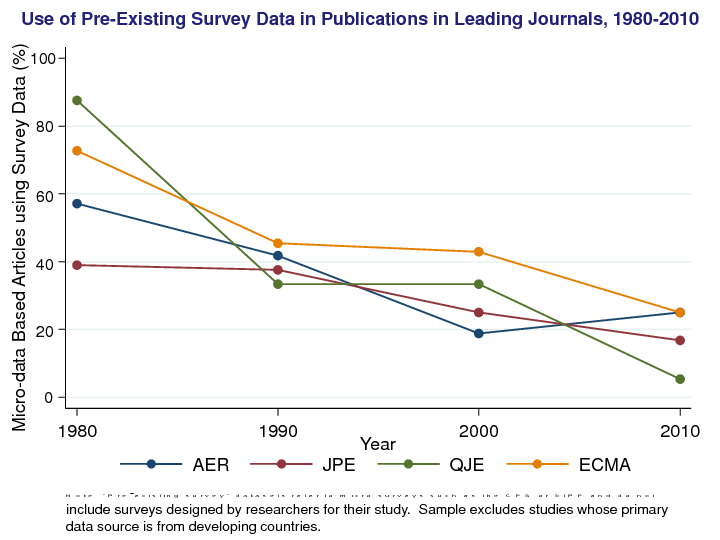
\includegraphics[width=0.7\paperwidth]{ChettySlide1}
\end{frame}

\begin{frame}
\frametitle{Increase in the use of administrative data in economics}
%\includepdf[pages={1-2}]{Chetty-1-2-Slides.pdf}
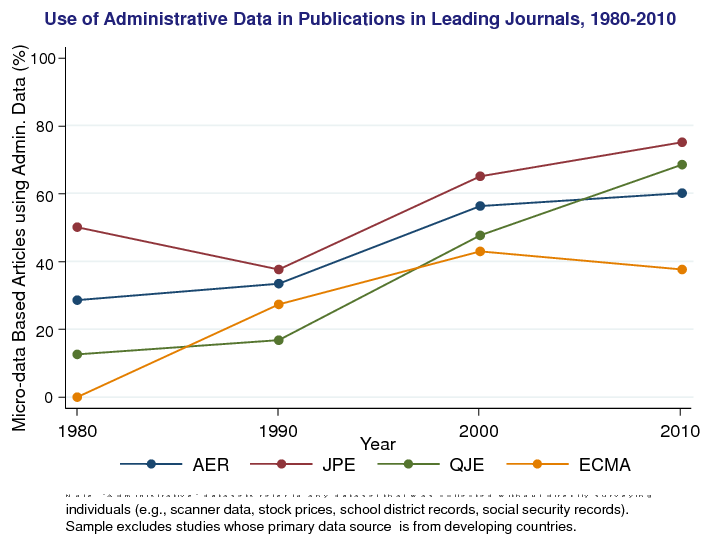
\includegraphics[width=0.7\paperwidth]{ChettySlide2}
\end{frame}

\begin{frame}
\frametitle{Not limited to economics}
\begin{block}{Nature, 2012}
``Many of the emerging `big data' applications come from private sources that are inaccessible to other researchers. The data source may be hidden, compounding problems of verification, as well as concerns about the generality of the results.''\\
\end{block}
{\tiny (Huberman, Nature 482, 308 (16 February 2012) \href{http://dx.doi.org/10.1038/482308d}{doi:10.1038/482308d})}
\begin{block}{Other domains}
\begin{itemize}
\item Biology (genetics data, chemical compounds)
\item Computer science (search records, single-firm examples)
\end{itemize}
\end{block}
\end{frame}

\section[Problem]{Stating the problem in the U.S. case}
\frame{\tableofcontents[currentsection]}

\begin{frame}
\frametitle{Why we think there is a problem}
\begin{block}{Core issues}
\begin{itemize}
\item[a] Insufficient curation (starting with archiving)
\item[b] No way to reference data (unique identifiers)
\item[c] No consistent way to learn about the data (metadata dissemination)
\item[d] Weak or non-existent provenance tracing
\end{itemize}
\end{block}
\end{frame}

\begin{frame}{Generalized problem}
\begin{block}{Multiple data sources in the US}
\begin{itemize}
\item U.S. Census Bureau (RDC) \hyperlink{Census}{\beamergotobutton{more}}
\item Internal Revenue Service (confidential, public-use)\hyperlink{IRS}{\beamergotobutton{more}}
\item Bureau of Labor Statistics (confidential, public-use data)\hyperlink{BLS}{\beamergotobutton{more}}

\end{itemize}
\end{block}
\begin{block}{Present elsewhere?}
\begin{itemize}
\item Canada: 
\begin{itemize}
\item Centre for Data Development and Economic Research (CDER: RDC-like for business data)\hyperlink{CDER}{\beamergotobutton{more}}
\item better: Canadian RDC network\hyperlink{CRDC}{\beamergotobutton{more}}
\end{itemize}
\item France:  R\'eseau Quetelet\hyperlink{France}{\beamergotobutton{more}}, Centre 
d'acc\'es s\'ecuris\'e distant aux donn\'ees (CASD) 
\item Germany: IAB
\end{itemize}
\end{block}
\end{frame}


%\begin{frame}
%\frametitle{Core problems}
%\begin{columns}
%  \begin{column}{0.3\textwidth}
%    \begin{itemize}[<+->]
%\item Curation\newline
%\item Identification\newline
%\item Information dissemination
%    \end{itemize}
%  \end{column}
%  \begin{column}{0.25\textwidth}
%  \begin{itemize}
%  \item[\ ]\onslide<4-6>{$\leftarrow$}\newline
%  \item[\ ]\onslide<5-6>{$\leftarrow$}\newline
%  \item[\ ]\onslide<6>{$\leftarrow$}\newline
%  \end{itemize}
%  \end{column}
%  \begin{column}{0.4\textwidth}
%     \begin{itemize}[<+->]
%        \item require cooperation of NSI
%        \item partial solution (DOI)\newline
%        \item core proposal\newline
%     \end{itemize}
%  \end{column}
%\end{columns}
%\end{frame}


\section[Solution]{CED$^2$AR: A proposed solution}
\frame{\tableofcontents[currentsection]}


\begin{frame}
\frametitle{Comprehensive Extensible Data Documentation and Access (CED$^2$AR)}
\begin{block}{Core}
We develop the core of a method for solving the data archive
and curation problem that confronts the custodians of restricted-access
research data and the scientific users of such data. Our solution recognizes 
the dual protections afforded by physical security and access limitation protocols, and allows for 
much improved provenance tracing.
\end{block}
\end{frame}

%\begin{frame}
%\frametitle{Requirements}
%\begin{block}{Royal Society (2012)}
%\begin{itemize}
%\item Accessible (a researcher can easily find it);
%\item Intelligible (to various audiences);
%\item Assessable (are researchers able make judgements about or
%assess the quality of the data);
%\item Usable (at minimum, by other scientists).
%\end{itemize}
%\end{block}
%\end{frame}


\begin{frame}
\frametitle{Proposed solution}
\begin{block}{Extensible framework}
\begin{itemize}[<+->]
\item Based on existing standards (\href{http://www.ddialliance.org}{Data Documentation 
Initiative}, DDI) with \alert<5>{extension to accomodate disclosure protection mechanisms and 
provenance tracing}
\item Connectors (import/export) to other sources and standards
\item To be filled by multiple sources of metadata (some the curators/owners, others ``crowd-sourced'')
\item Interim solution for those datasets without unique identifiers 
(\href{http://datacite.org/whatisdoi}{Digital Object Identifier}, DOI)
\end{itemize}
\end{block}
\end{frame}

\begin{frame}
\vfill 
\centering What is DDI?
\vfill
\end{frame}

%\begin{frame}
%\frametitle{Extensions to DDI}
%\begin{block}{Basic idea}
%\begin{tabular}{rcl}
%\only<1>{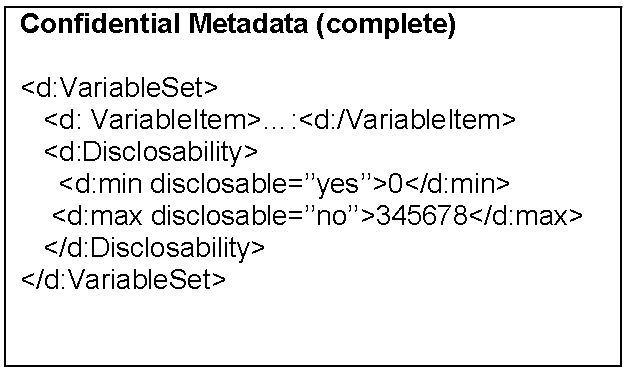
\includegraphics[width=0.4\textwidth]{ConfidentialMetadata-left}}
%\only<2->{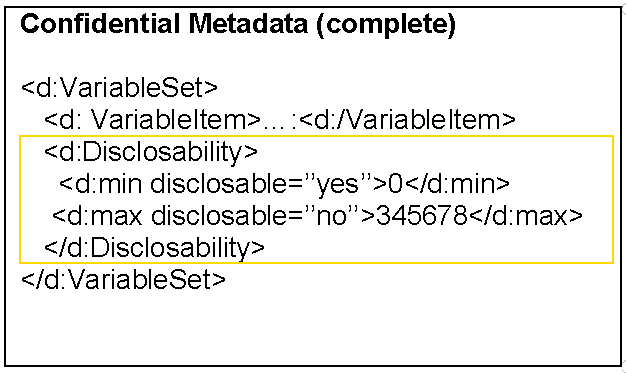
\includegraphics[width=0.4\textwidth]{ConfidentialMetadata-left-hilite}}\pause \pause &
%
\includegraphics[width=0.1\textwidth]{wall-export-small}&
%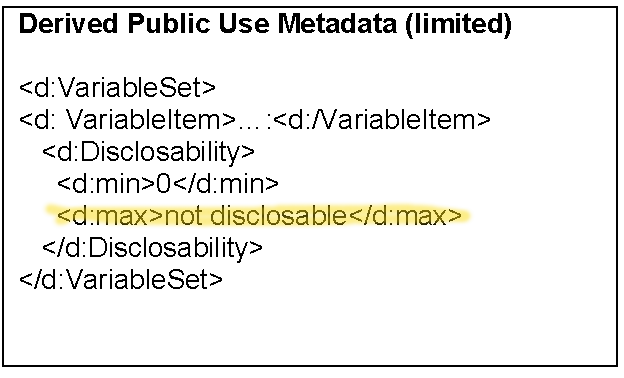
\includegraphics[width=0.4\textwidth]{ConfidentialMetadata-right}
%\end{tabular}
%\end{block}
%\end{frame}

%\begin{frame}
%\frametitle{Database design}
%\begin{block}{Multiple sources}
%\begin{itemize}
%\item Data-curator-provided metadata (possibly regularly updated, PRUNED)
%\item Alternate sources (IPUMS data to describe Decennial Census)
%\item {\bf User-provided metadata (wiki) (planned fall 2013)}
%\end{itemize}
%\end{block}
%\begin{block}{Multiple outputs}
%\begin{itemize}
%\item Local query ({\bf working})
%\item Remote federation or export
%\item Synchronization back to data-curator (data enclave!)
%\end{itemize}
%\end{block}
%\end{frame}

\subsection[DDI]{What is DDI}

\begin{frame}[fragile]{Example of DDI}
\begin{minted}[fontsize=\footnotesize]{xml}
<?xml version="1.0" encoding="UTF-8"?>
<codeBook xmlns="ddi:codebook:2_5" ...>
   <docDscr>
      <citation>
         <titlStmt>
           <titl>SIPP_Synthetic_Beta</titl>
           <altTitl>SSB</altTitl>
           <IDNo agency="DOI">TBD</IDNo>
         </titlStmt>
         <rspStmt>
            <AuthEnty affiliation="Cornell University">
               Virtual RDC
            </AuthEnty>
          </rspStmt>
\end{minted}
\end{frame}

\begin{frame}{..better seen as}
\begin{center}
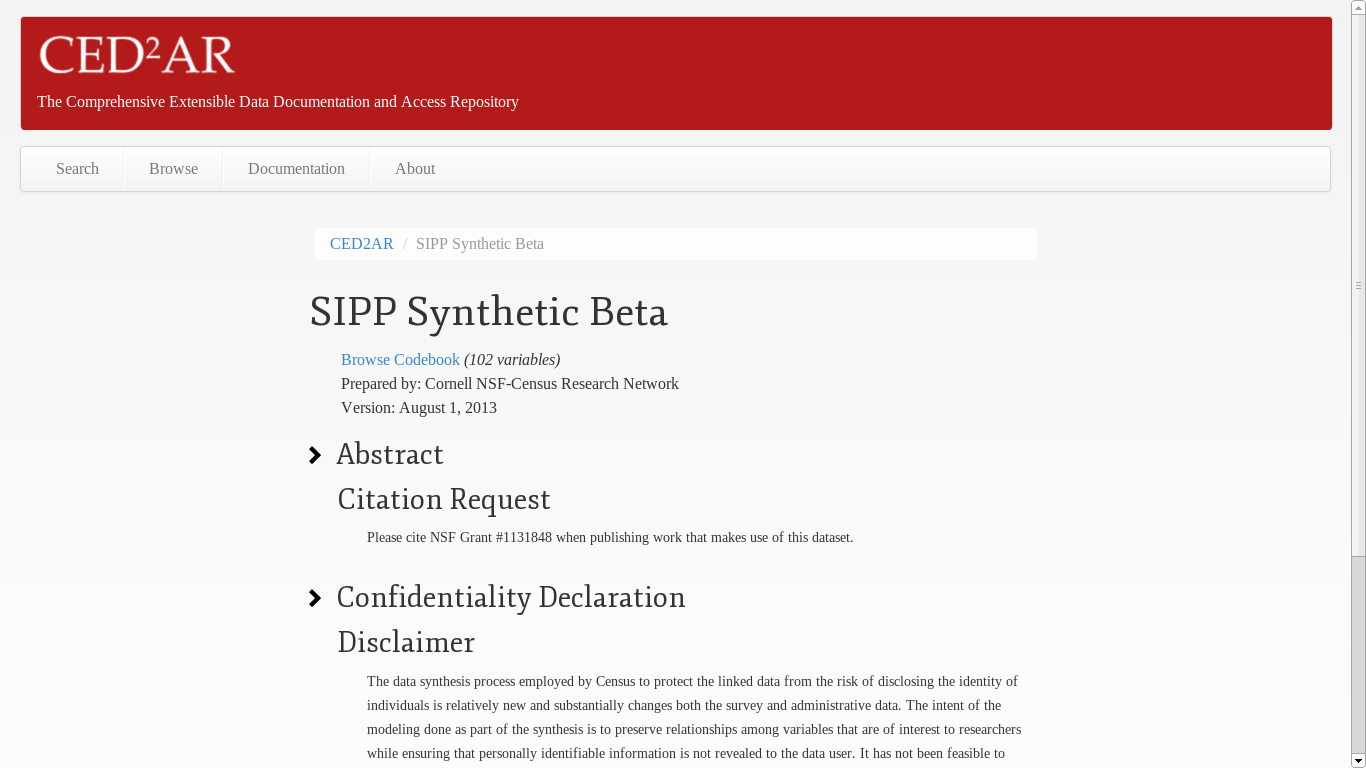
\includegraphics[width=0.9\linewidth]{ced2ar-ssb}
\end{center}
\end{frame}

\begin{frame}{Example DDI: ICPSR}
\begin{center}
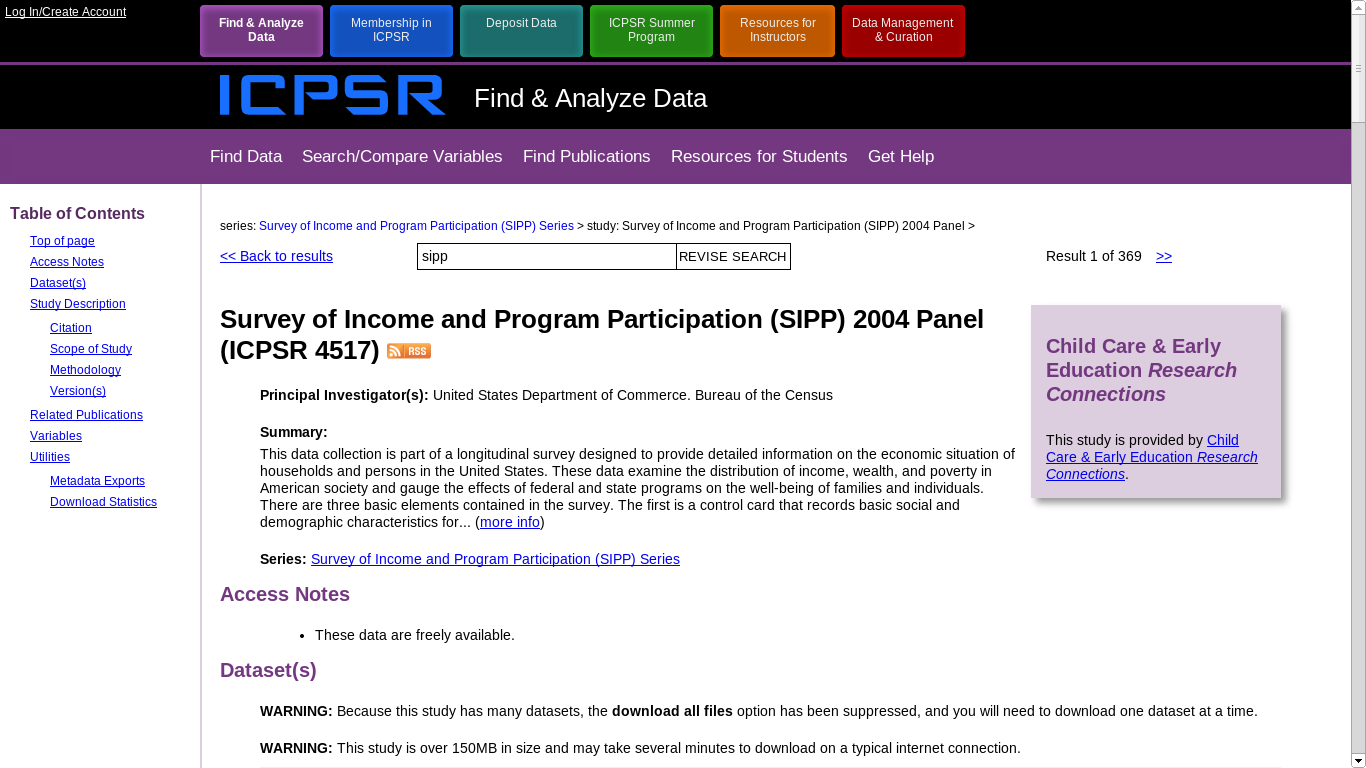
\includegraphics[width=0.9\linewidth]{icpsr}
\end{center}
\end{frame}

\begin{frame}{Example DDI: UK data archive}
\begin{center}
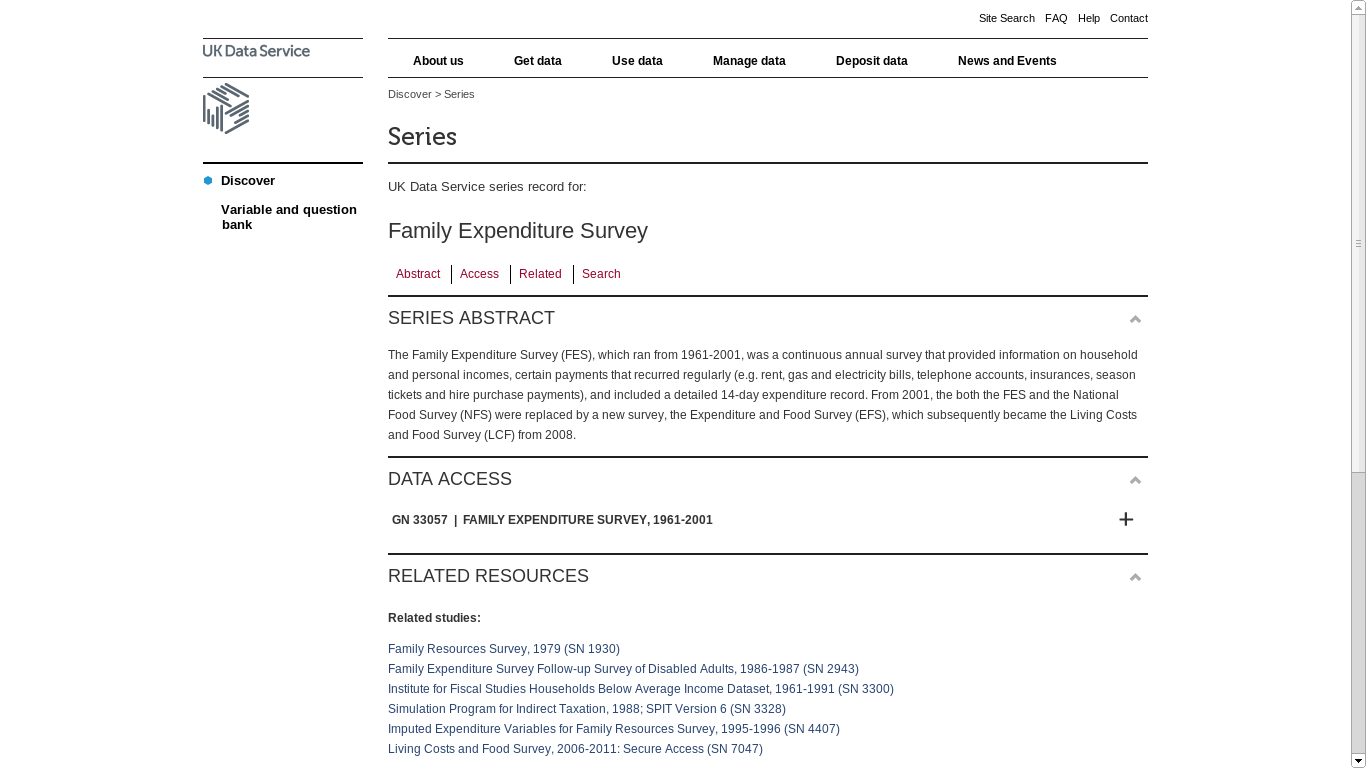
\includegraphics[width=0.9\linewidth]{uk_data_archive}
\end{center}
\end{frame}

\subsection[Confidentiality]{DDI extension for confidentiality protection}

\begin{frame}[fragile]{Expanded DDI attributes}
\begin{block}{Standard DDI}
Fragment of variable description$^*$
\begin{minted}[fontsize=\footnotesize]{xml}
   <var ID="V1" dcml="0" files="F1" intrvl="discrete" 
   			name="cur_end mar_flag">
       <location width="12"/>
         <labl>Flag: Linked marriage ended</labl>
           <valrng>
             <range UNITS="REAL" max="2" min="0"/>
           </valrng>
           <sumStat type="vald"> 123 </sumStat>
           <sumStat type="invd"> 456 </sumStat>
           <catgry>
             <catValu> 1 </catValu>
             <catStat type="freq"> 234 </catStat>
           </catgry>
\end{minted}
\end{block}
\tiny{$^*$ All values are fake}
\end{frame}

\begin{frame}[fragile]{Expanded DDI attributes}
\begin{block}{Standard DDI}
Fragment of variable description$^*$
\begin{minted}[fontsize=\footnotesize]{xml}
   <!--var ID="V1" dcml="0" files="F1" intrvl="discrete" 
   			name="cur_end mar_flag">
       <location width="12"/>
         <labl>Flag: Linked marriage ended</labl -->
           <valrng>
             <range UNITS="REAL" max="2" min="0"/>
           </valrng>
           <!-- sumStat type="vald"> 123 </sumStat>
           <sumStat type="invd"> 456 </sumStat>
           <catgry>
             <catValu> 1 </catValu>
             <catStat type="freq"> 234 </catStat>
           </catgry -->
\end{minted}
\end{block}
\tiny{$^*$ All values are fake}
\end{frame}

\begin{frame}[fragile]{Expanded DDI attributes}
\begin{block}{Standard DDI}
Fragment of variable description$^*$
\begin{minted}[fontsize=\footnotesize]{xml}
   <!--var ID="V1" dcml="0" files="F1" intrvl="discrete" 
   			name="cur_end mar_flag">
       <location width="12"/>
         <labl>Flag: Linked marriage ended</labl>
           <valrng>
             <range UNITS="REAL" max="2" min="0"/>
           </valrng -->
           <sumStat type="vald"> 123 </sumStat>
           <sumStat type="invd"> 456 </sumStat>
           <!-- catgry>
             <catValu> 1 </catValu>
             <catStat type="freq"> 234 </catStat>
           </catgry -->
\end{minted}
\end{block}
\tiny{$^*$ All values are fake}
\end{frame}



\begin{frame}[fragile]{Expanded DDI attributes}

\begin{block}{Enhanced DDI}
Re-using existing attribute, but expanding scope.$^*$
\begin{minted}[fontsize=\footnotesize]{xml}
   <var ID="V1" dcml="0" files="F1" intrvl="discrete" 
   			name="cur_end mar_flag">
       <location width="12"/>
         <labl>Flag: Linked marriage ended</labl>
           <valrng access="release">
             <range UNITS="REAL" max="2" min="0"/>
           </valrng>
           <sumStat access="restricted" type="vald"> 123 </sumStat>
           <sumStat access="restricted" type="invd"> 456 </sumStat>
           <catgry access="release">
             <catValu access="release"> 1 </catValu>
             <catStat type="freq" access="restricted"> 
                  234
             </catStat>
           </catgry>
\end{minted}
\end{block}
\tiny{$^*$ All values are fake}
\end{frame}

\begin{frame}[fragile]{Expanded DDI attributes}

\begin{block}{Enhanced DDI}
Allows for verifiable filtering$^*$
\begin{minted}[fontsize=\footnotesize]{xml}
   <var ID="V1" dcml="0" files="F1" intrvl="discrete" 
   			name="cur_end mar_flag">
       <location width="12"/>
         <labl>Flag: Linked marriage ended</labl>
           <valrng access="release">
             <range UNITS="REAL" max="2" min="0"/>
           </valrng>
           <!-- sumStat suppressed -->
           <!-- sumStat suppressed -->
           <catgry access="release">
             <catValu access="release"> 1 </catValu>
             <catStat type="freq" access="restricted"> 
                  [suppressed]
             </catStat>
           </catgry>
\end{minted}
\end{block}
\tiny{$^*$ All values are fake}
\end{frame}


\begin{frame}{Application to confidentiality protection}
\begin{center}
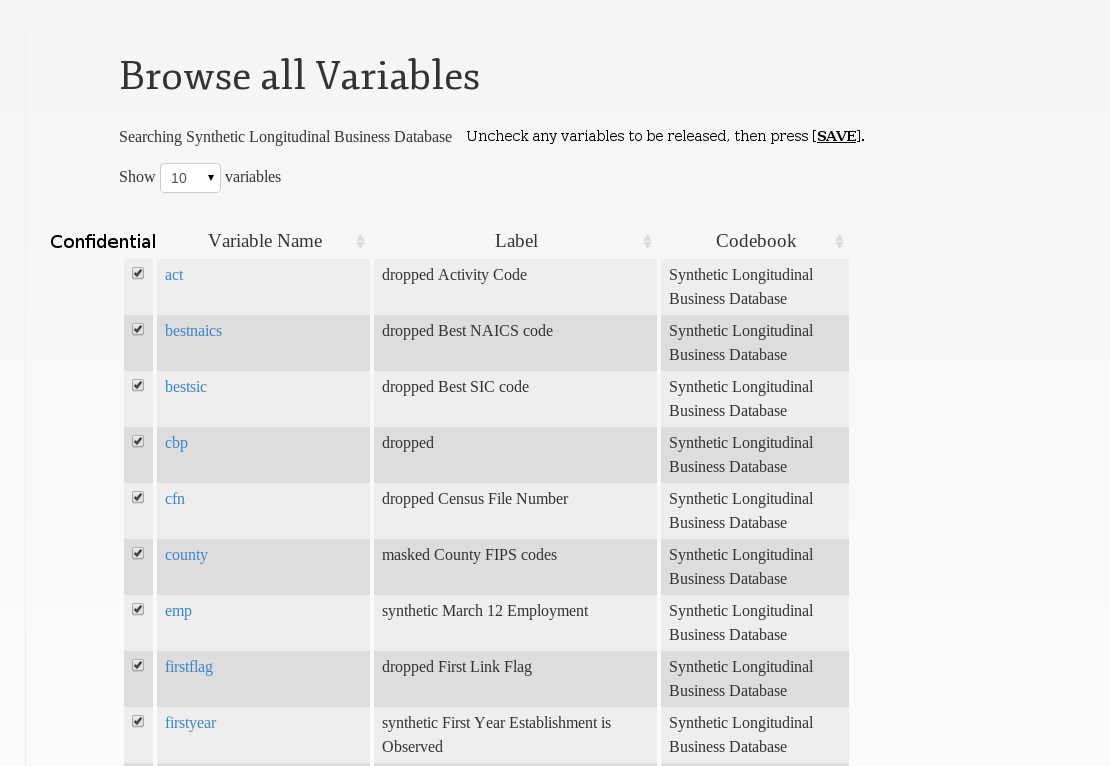
\includegraphics[width=1\linewidth]{Screenshot_2013-11-04_13:18:01_mockup}
\end{center}
\end{frame}

\begin{frame}[fragile]{Options}
\begin{itemize}
\item Variable is suppressed, including all subordinate elements
\item Variable description is released, but all subordinate statistical elements are suppressed
          (attribute of $<var>$ set to "released") [default]
\item Expand all existing attributes, individually select subordinate elements to suppress 
(attribute of sub-element is set to "suppressed", content suppressed)
\end{itemize}
\end{frame}


\begin{frame}{Application to confidentiality protection}
\begin{center}
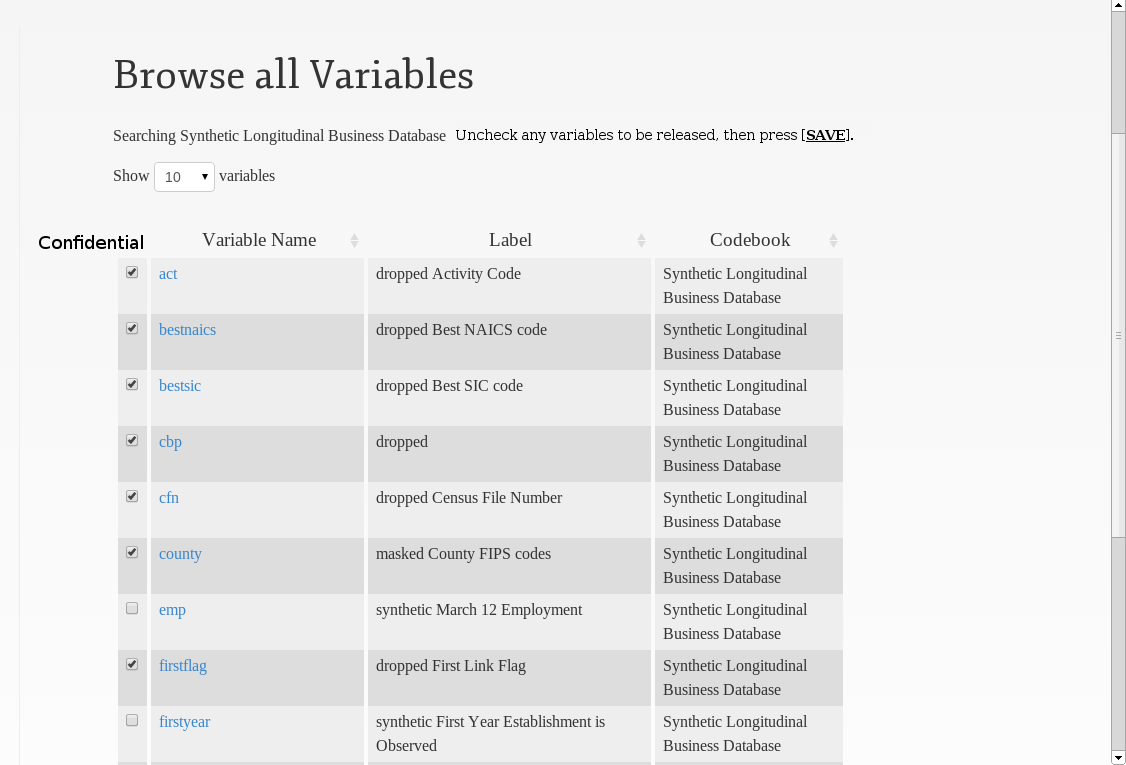
\includegraphics[width=1\linewidth]{Screenshot_2013-11-04_13:18:11_mock}
\end{center}
\end{frame}

\begin{frame}{Application to confidentiality protection}
\begin{center}
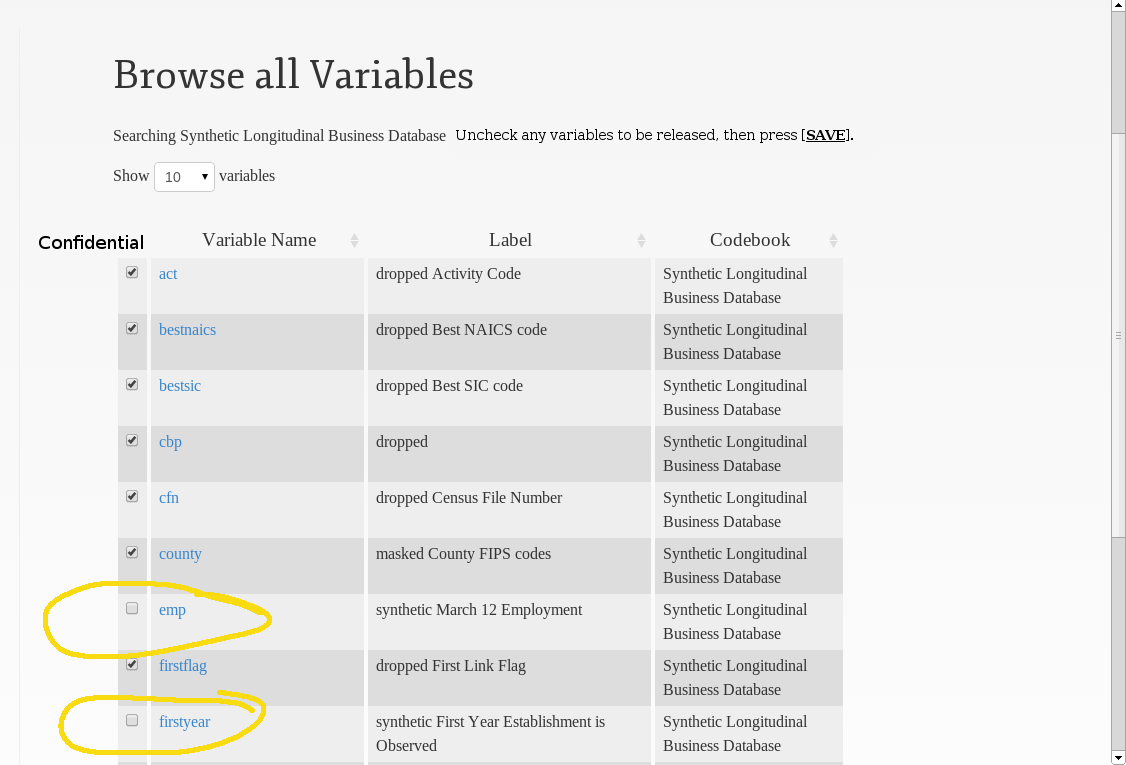
\includegraphics[width=1\linewidth]{Screenshot_2013-11-04_13:18:11_mock2}
\end{center}
\end{frame}

\begin{frame}{Implementation}
\begin{block}{Definitions}
\begin{itemize}[<+->]
\item First draft of specification in test use by our team
\item Full enhanced specification (based on DDI-Codebook 2.5) published on CED$^2$AR
\item Enhanced specification proposed to DDI Alliance
\item Expand to DDI-Lifecycle
\end{itemize}
\end{block}
\end{frame}

\subsection[Provenance]{DDI extension for provenance tracing}
\begin{frame}{Provenance}
\begin{block}{The provenance problem}
``data provenance, one kind of metadata, pertains to the derivation history of a
data product starting from its original sources'' [...]  ``from it, one can ascertain
the quality of the data base and its ancestral data and derivations, track back sources
of errors, allow automated reenactment of derivations to update the data, and provide 
attribution of data sources'' 
\end{block}
{\tiny Simmhan, Plale, and Gannon, ``A survey of data provenance in e-science,'' ACM Sigmod Record, 2005}
\end{frame}

\begin{frame}[fragile]{Support in DDI}
\begin{block}{Provenance and Metadata}
Not (currently) a ``native'' component of DDI, closest thing is:
\begin{minted}[fontsize=\tiny,gobble=3]{xml}
   <xs:complexType name="othrStdyMatType">
      <xs:complexContent>
         <xs:extension base="baseElementType">
            <xs:sequence>
               <xs:element ref="relMat" minOccurs="0" maxOccurs="unbounded"/>
               <xs:element ref="relStdy" minOccurs="0" maxOccurs="unbounded"/>
               <xs:element ref="relPubl" minOccurs="0" maxOccurs="unbounded"/>
               <xs:element ref="othRefs" minOccurs="0" maxOccurs="unbounded"/>
            </xs:sequence>
         </xs:extension>
      </xs:complexContent>
   </xs:complexType>
\end{minted}
\end{block}
\begin{block}{Downside}
No structure. Mostly verbose entries.
\end{block}
\end{frame}

\begin{frame}{Only a verbose description}
\begin{center}
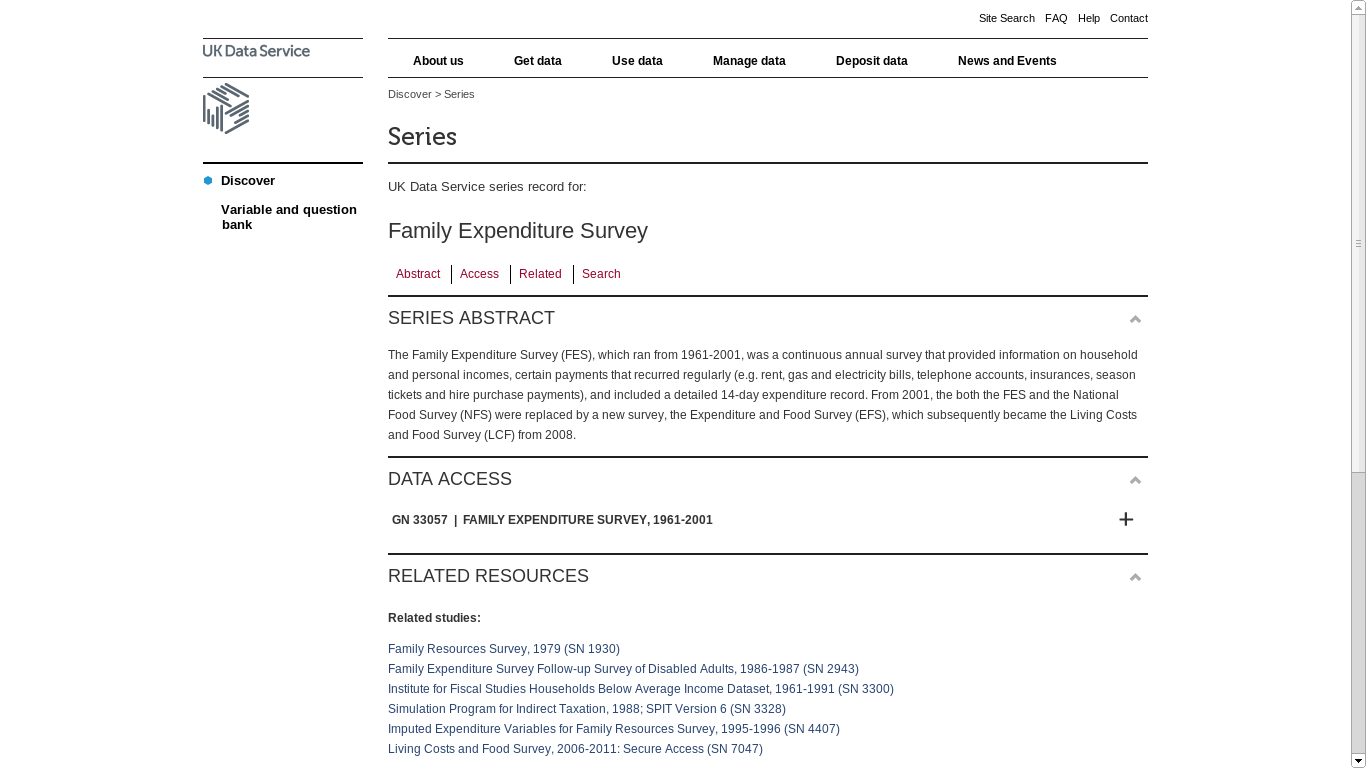
\includegraphics[width=1\linewidth]{uk_data_archive}
\end{center}
\end{frame}

\begin{frame}{UK Data Archive example}
\begin{center}
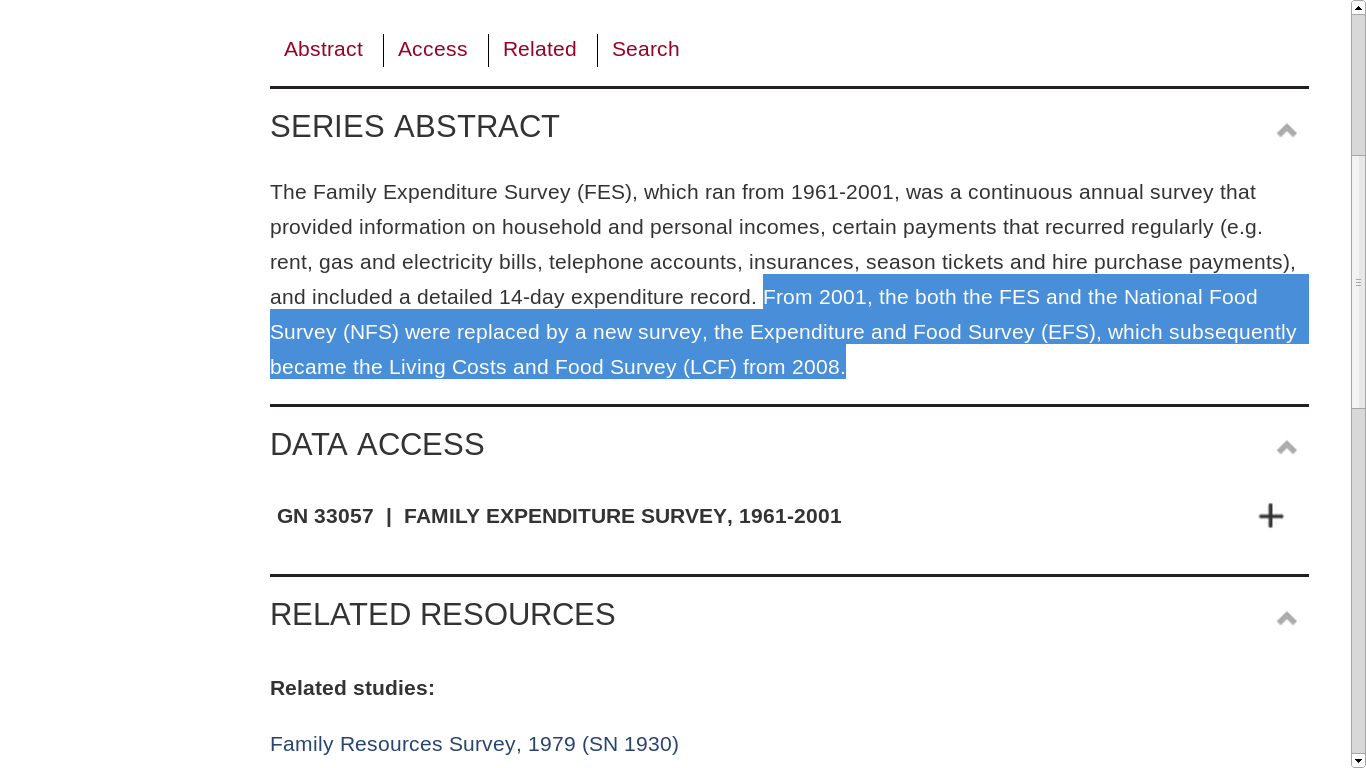
\includegraphics[width=1\linewidth]{uk_data_archive_zoom}
\end{center}
\end{frame}


\begin{frame}{Provenance (cont)}
\begin{block}{PROV model}
W3C PROV Model  based in the notions of 
\begin{enumerate}
\item \textbf{entities} that are physical, digital, and conceptual
things in the world; 
\item \textbf{activities} that are dynamic aspects of the world that change and
create entities; and 
\item \textbf{agents} that are responsible for activities. 
\item  a set of \textbf{relationships} that can exist be-
tween them that express attribution,. delegation, derivation, etc.
\end{enumerate}
\end{block}
\end{frame}

\begin{frame}{Incorporating PROV (LBD)}
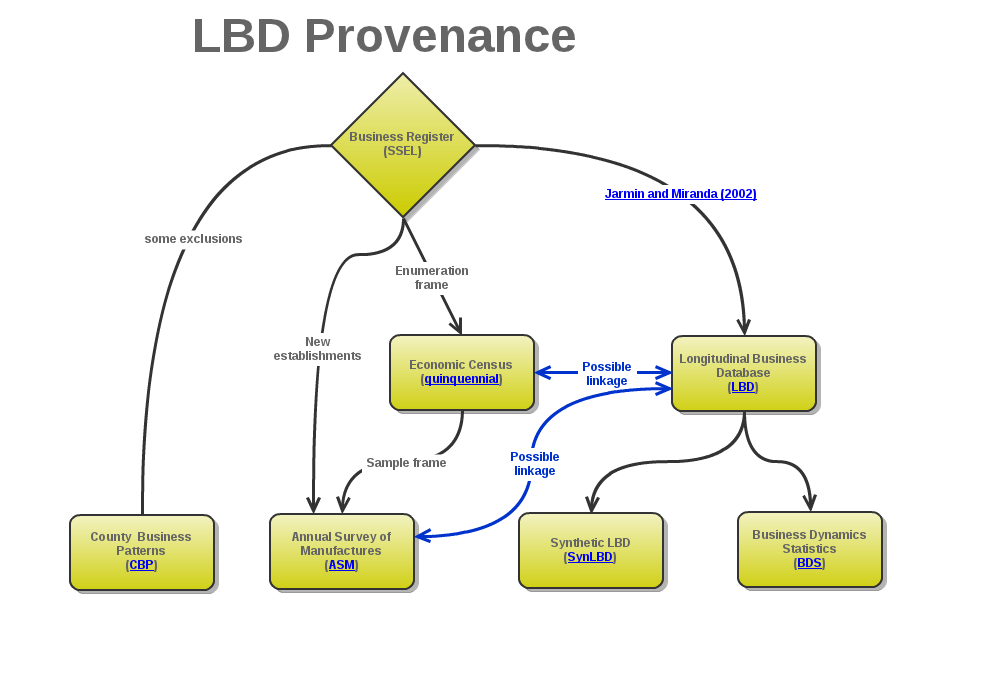
\includegraphics[width=\textwidth]{LBD_Provenance.png}
\end{frame}

\begin{frame}{Incorporating PROV (LBD)}
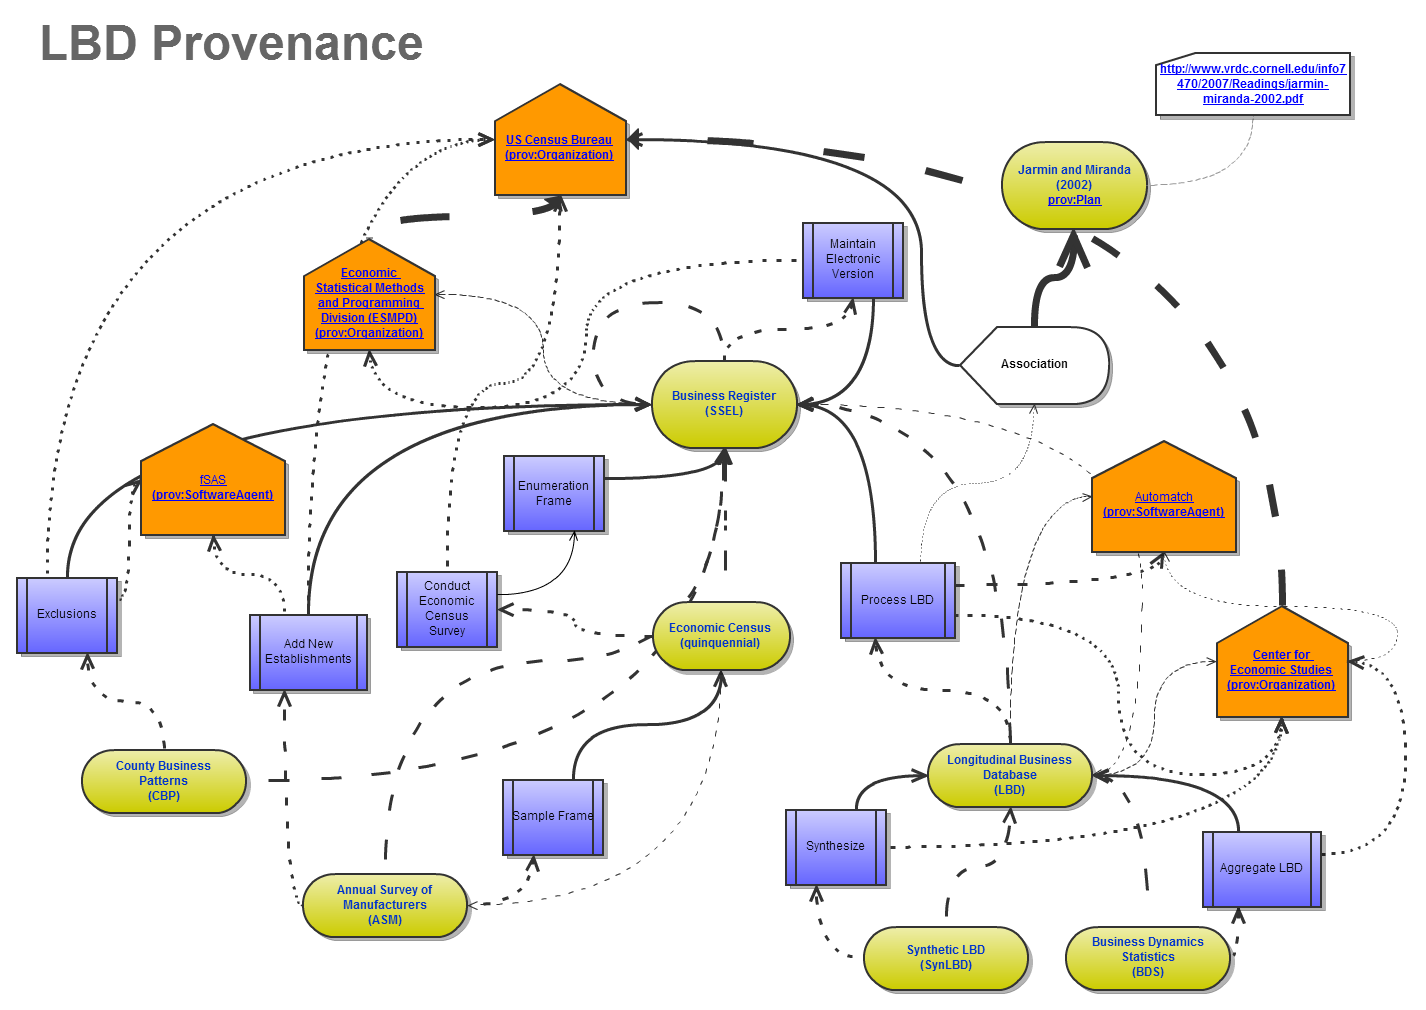
\includegraphics[width=0.9\textwidth]{LBD_PROV_-_WIP.png}
\end{frame}

\begin{frame}{Incorporating PROV (LBD)}
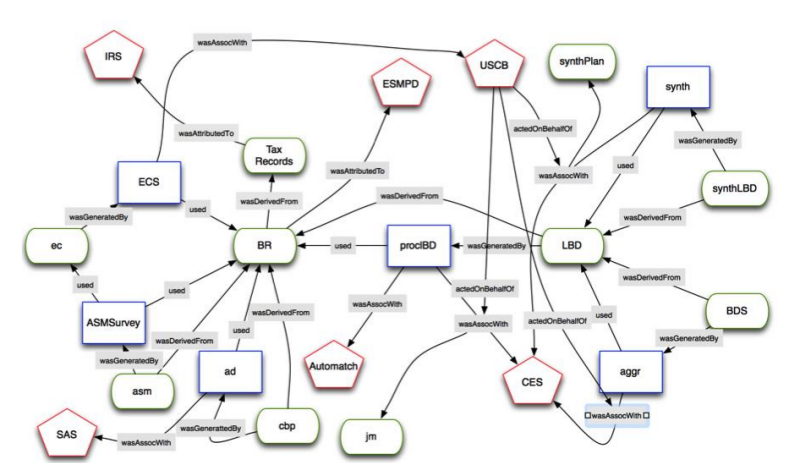
\includegraphics[width=0.9\textwidth]{LBD_Prov_simplified.png}
\end{frame}

\begin{frame}{PROV as RDF}
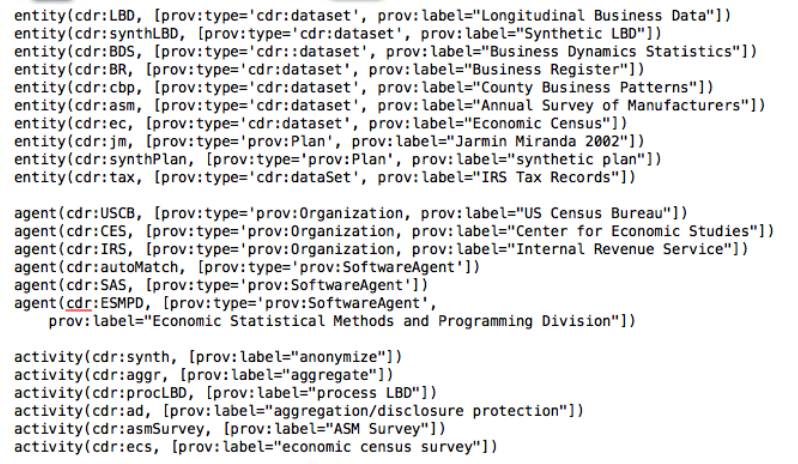
\includegraphics[width=0.9\textwidth]{LBD_Prov_simplified_text.png}
\end{frame}

\begin{frame}[fragile]{}
\begin{block}{The key PROV element embedded as DDI/XML}
\begin{minted}[fontsize=\footnotesize]{xml}
<stdyDscr> <!-- Standard DDI 2.5 -->
 <othrStdyMat> <!-- Standard DDI 2.5 -->
  <relStdy>  <!-- Standard DDI 2.5 -->
     <!-- From here, PROV additions -->
    <prov:wasDerivedFrom>
        <prov:generatedEntity prov:ref="cdr:LBD"/>
        <prov:usedEntity prov:ref="cdr:BR"/>
    </prov:wasDerivedFrom>
     <prov:wasAssociatedWith>
          <prov:activity prov:ref="cdr:procLBD"/>
          <prov:agent prov:ref="cdr:CES"/>
          <prov:plan prov:ref="cdr:procLBDPlan"/>
        </prov:wasAssociatedWith>     
  </relStdy> <!-- Standard DDI 2.5 -->
 </othrStdyMat> <!-- Standard DDI 2.5 -->
</stdyDscr><!-- Standard DDI 2.5 -->
\end{minted}
\end{block}
\end{frame}

\begin{frame}[fragile]
\begin{block}{Additional PROV elements}
These could be derived from existing DDI elements (still being developed)
\begin{minted}[fontsize=\footnotesize]{xml}
     <!-- Entities -->
    <prov:entity prov:id="cdr:BR">
        <dct:title>Business Register</dct:title>
    </prov:entity>
    <!-- Plans = Methodology -->
     <prov:plan prov:id="cdr:procLBDPlan">       
        <prov:location 
        xsi:type="xsd:anyURI">
        http://ideas.repec.org/p/cen/wpaper/02-17.html
        </prov:location>
        <prov:type>prov:Plan</prov:type>
    </prov:plan>
\end{minted}
\end{block}
\end{frame}




\begin{frame}{Work on PROV}
\begin{block}{More details forthcoming}
\begin{itemize}
\item Lagoze, Williams, Vilhuber ``Encoding Provenance Metadata for
Social Science Datasets'', submitted to Metadata and Semantics Research Conference 
(November 2013)
\item Lagoze, Williams, Vilhuber, Block ``Encoding Provenance of Social Science Data: 
Integrating PROV with DDI'', accepted for 5th Annual European DDI User Conference 
(December 2013)
\end{itemize}
\end{block}
\end{frame}


%\begin{frame}
%\frametitle{State of the implementation}
%\begin{block}{DDI extension}
%Being incorporated.
%\end{block}
%\begin{block}{DOI assignment}
%Our project (NCRN) will assign/register DOI if not provided by curator/owner
%\end{block}
%\begin{block}{Database}
%Design finalized, database populated with  metadata for newest SIPP Synthetic Beta. Wiki 
%additions  Fall 2013
%\end{block}
%\begin{block}{UI}
%Version 1.1 of the UI being completed (more robust, scalable). Wiki additions in Fall 2013
%\end{block}
%\begin{block}{Provenance}
%PROV extension, integration Winter 2013/14
%\end{block}
%\end{frame}

\begin{frame}{Usage scenario}
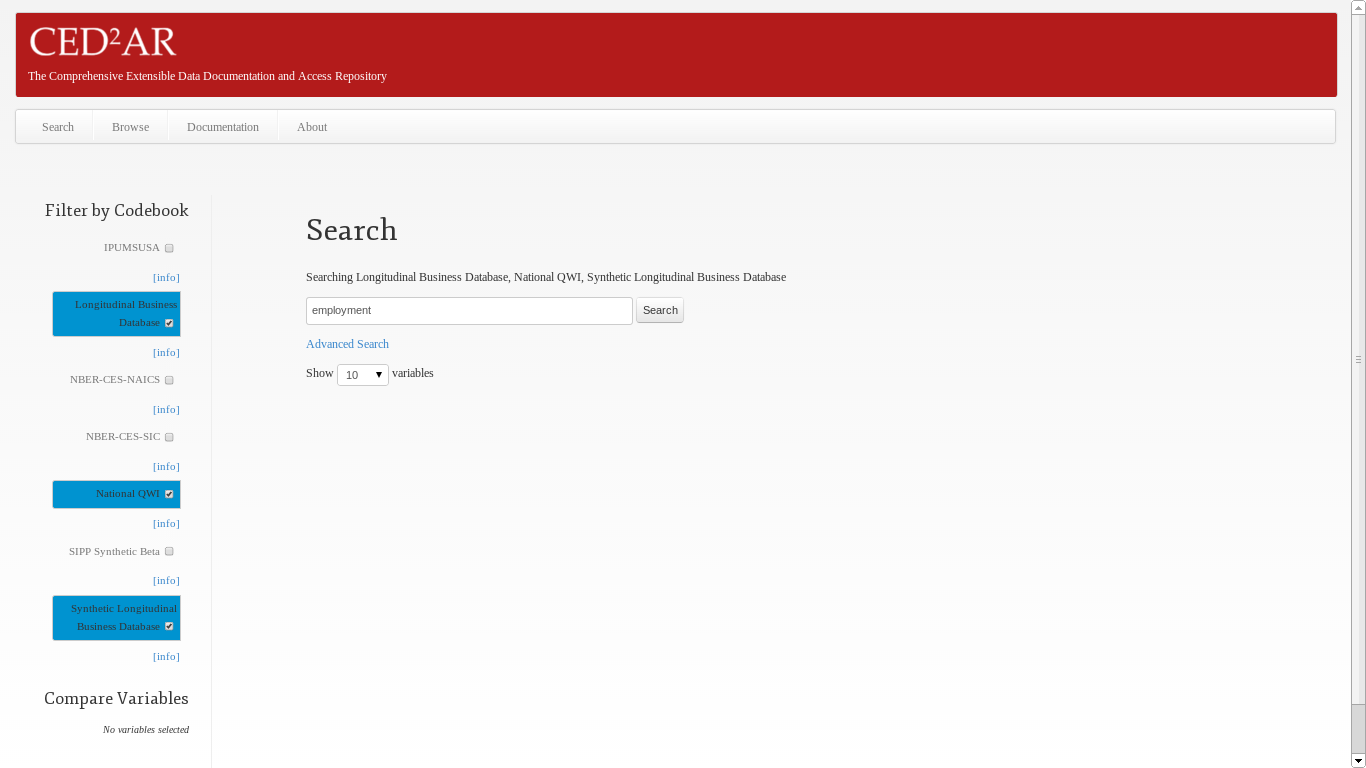
\includegraphics[width=1.1\linewidth]{Screenshot_2013-11-04_12:42:19.png}
\end{frame}
\begin{frame}{Usage scenario}
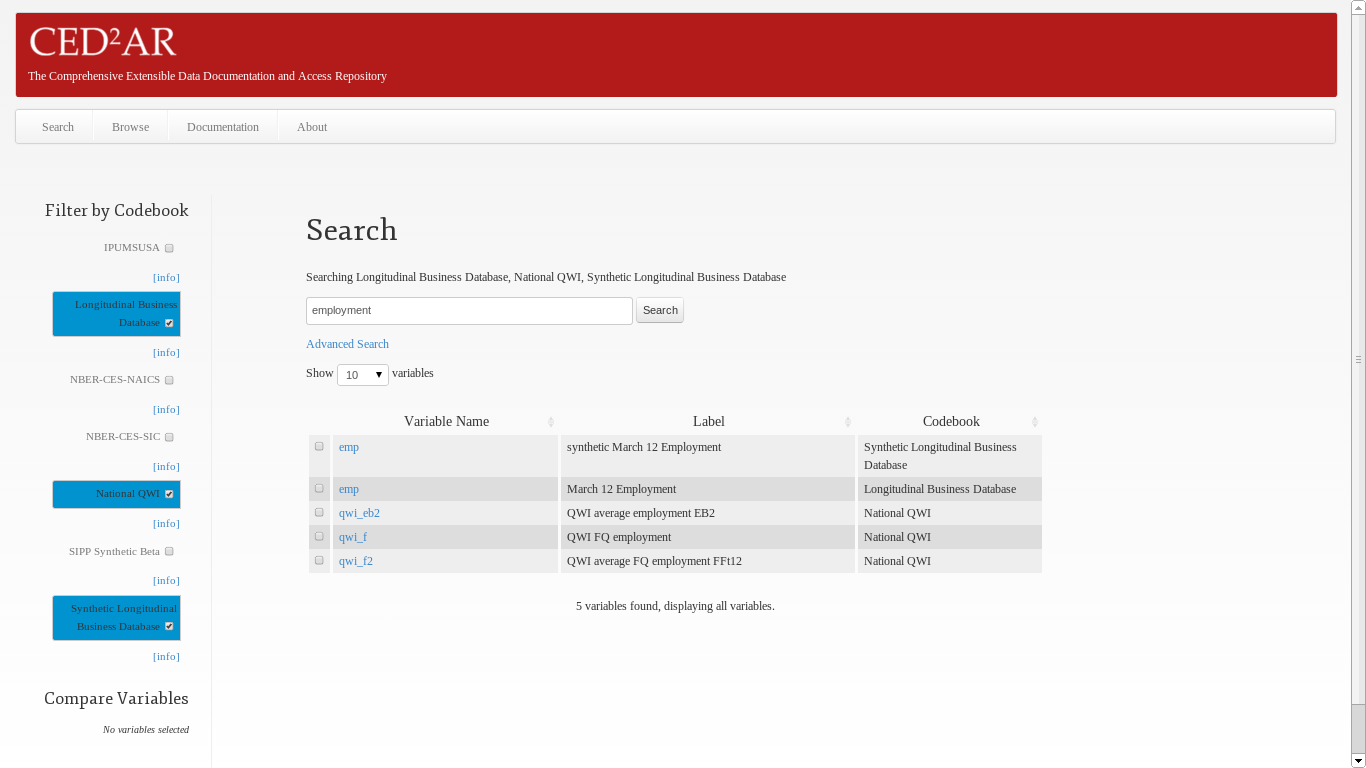
\includegraphics[width=1.1\linewidth]{Screenshot_2013-11-04_12:42:24.png}
\end{frame}
\begin{frame}{Usage scenario}
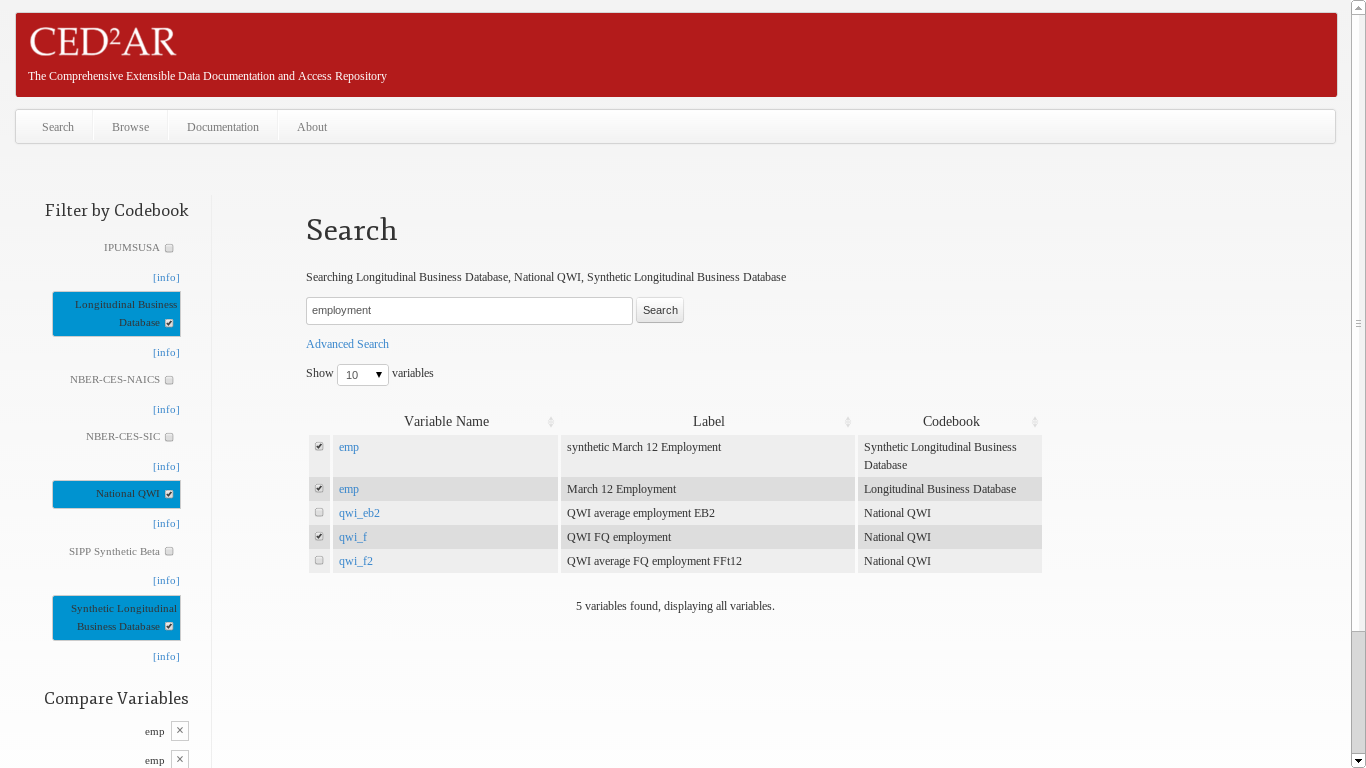
\includegraphics[width=1.1\textwidth]{Screenshot_2013-11-04_12:42:38.png}
\end{frame}
\begin{frame}{Usage scenario}
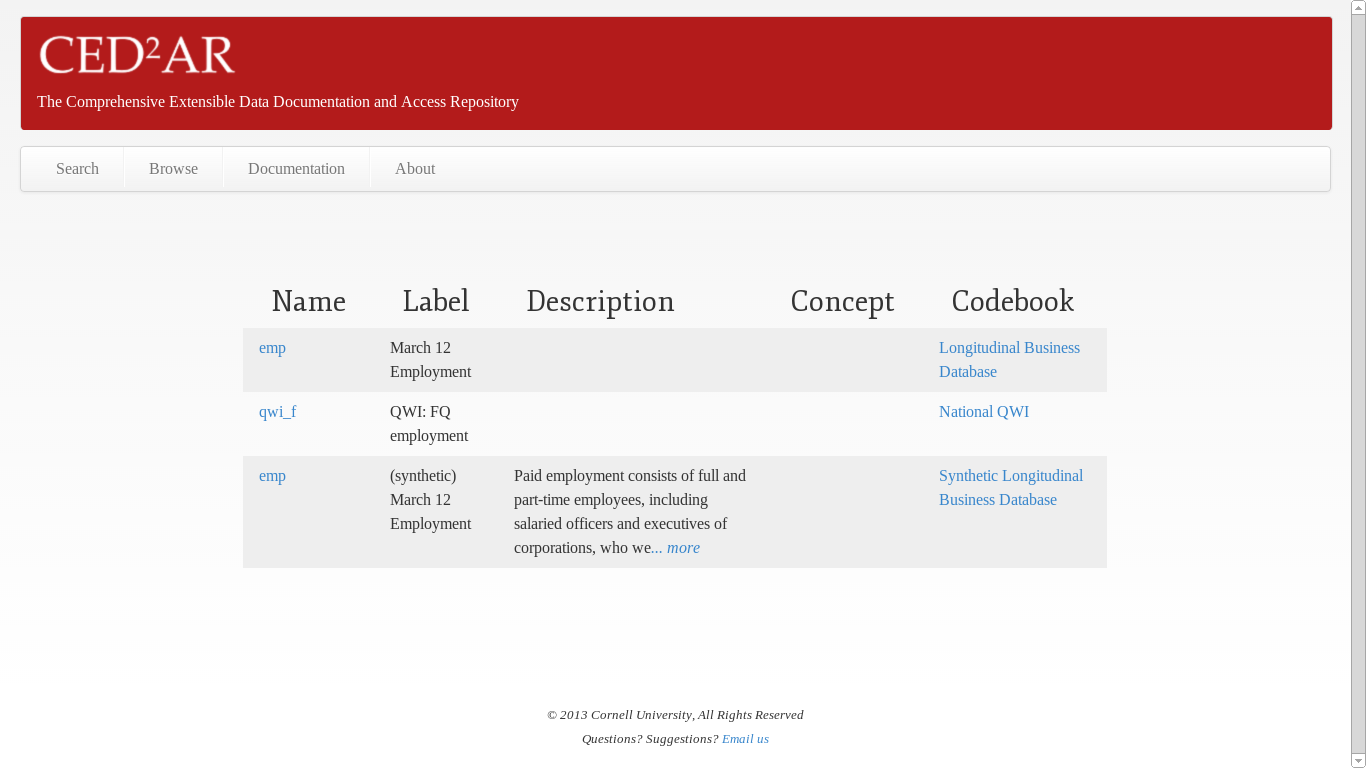
\includegraphics[width=1.1\textwidth]{Screenshot_2013-11-04_12:43:01.png}
\end{frame}
\begin{frame}{Highlighting provenance}
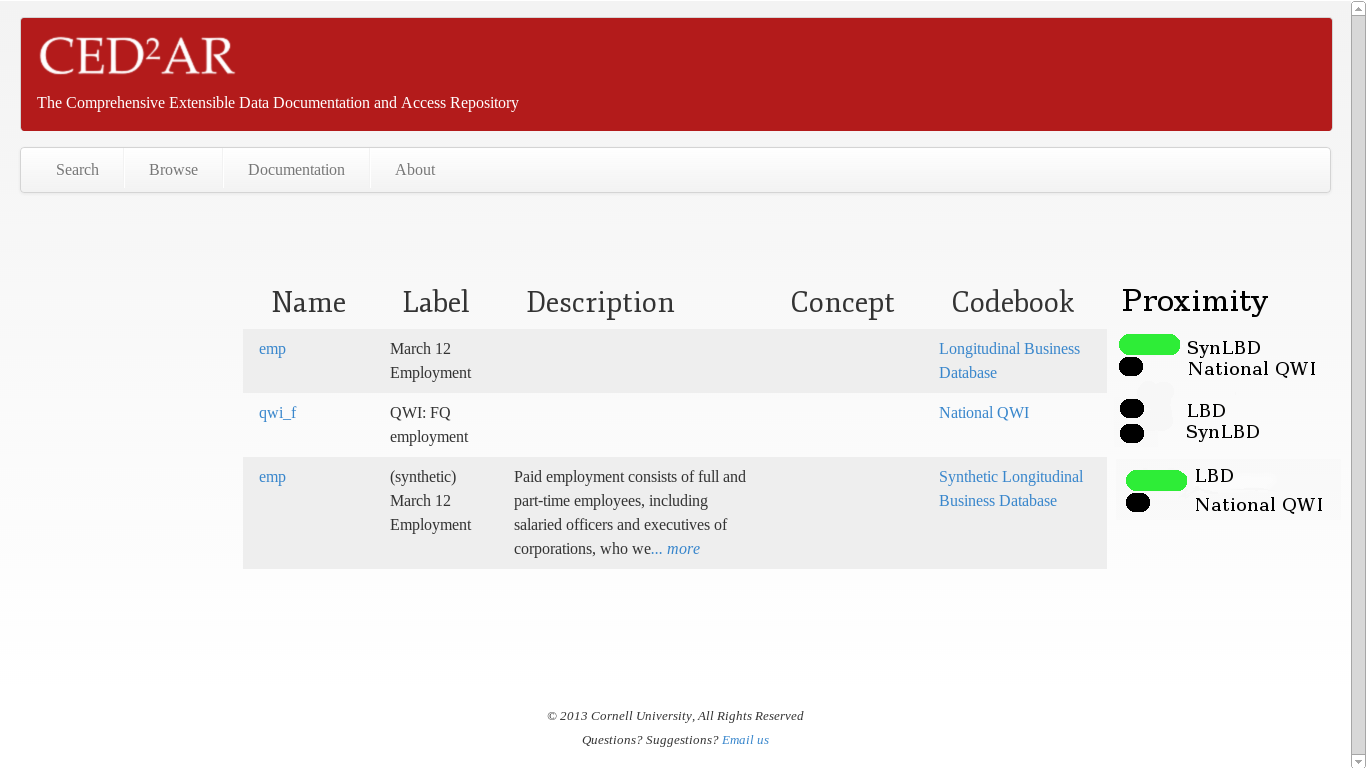
\includegraphics[width=1.1\textwidth]{Screenshot_2013-11-04_12:43:01-prov.png}
\end{frame}


\begin{frame}{CED$^2$AR next steps}
\begin{itemize}[<+->]
\item Formalize the DDI extension
\item Provide implementation outside of Census Bureau
\item Test implementation within the Census RDC
\end{itemize}
\end{frame}

\section*{Additional info}
\begin{slide}
\frametitle{The end}
\begin{block}{Thank you}
\begin{itemize}
\item \cite{AbowdVilhuberBlock2012} for more details
\item \href{http://www.ilr.cornell.edu/LDI/}{Labor Dynamics Institute}
\item \href{http://www.vrdc.cornell.edu}{VirtualRDC @ Cornell}
\item \href{http://www.ncrn.cornell.edu/}{NCRN Cornell website}
\end{itemize}
\end{block}
\end{slide}

\begin{frame}[fragile]
\begin{verbatim}
$Id: Presentation-FCSM2013-subdoc.tex 406 2013-11-05 03:23:30Z lv39 $
\end{verbatim}
\end{frame}

%%% Local Variables:
%%% mode: latex
%%% End:
